%Este trabalho está licenciado sob a Licença Atribuição-CompartilhaIgual 4.0 Internacional Creative Commons. Para visualizar uma cópia desta licença, visite http://creativecommons.org/licenses/by-sa/4.0/deed.pt_BR ou mande uma carta para Creative Commons, PO Box 1866, Mountain View, CA 94042, USA.

\chapter{Fundamentos}\label{cap_vetor}

Neste capítulo, seguimos uma abordagem geométrica para introduzir os conceitos fundamentais e as operações básicas envolvendo vetores.

\section{Segmentos Orientados}\label{cap_vetor_sec_segorien}

O conceito de \hl{\emph{segmento orientado}} é fundamental na definição de vetores. Como o próprio nome indica, \hl{trata-se de definir uma orientação a um dado \emph{segmento de reta}}. Antes, portanto, vamos definir o que entendemos por um segmento.

\subsection{Segmento}
\badgeYouTube{https://www.youtube.com/embed/J-GN-uulfRs}

\hl{Sejam dados dois pontos $A$ e $B$ sobre uma reta $r$. O conjunto de todos os pontos de $r$ entre $A$ e $B$ é chamado de \emph{segmento} e denotado por $AB$.} A reta $r$ é chamada de \emph{reta suporte} e os pontos $A$ e $B$ de \emph{pontos extremos}. Consulte a Figura~\ref{cap_vetor_sec_segorien:fig:segmento}.

\begin{figure}[h]
  \centering
  \includegraphics{./cap_vetor/dados/fig_segmento/fig.png}
  \caption{Um segmento $AB$ de uma reta (direção) $r$.}
  \label{cap_vetor_sec_segorien:fig:segmento}
\end{figure}

\subsubsection{Comprimento e Direção}

\hl{O \emph{comprimento} de um segmento $AB$ é denotado por $|AB|$ e definido como a distância entre seus pontos extremos $A$ e $B$}. Em outras palavras, é o tamanho do segmento\footnote{Em aplicações, o comprimento é medido em unidades de comprimento, metro $(m)$, no sistema internacional de unidades (SI).}. Consulte a Figura~\ref{cap_vetor_sec_segorien:fig:segmento_norma}

\begin{figure}[h]
  \centering
  \includegraphics{./cap_vetor/dados/fig_segmento_norma/fig.png}
  \caption{Comprimento de um segmento $AB$.}
  \label{cap_vetor_sec_segorien:fig:segmento_norma}
\end{figure}

\hl{A \emph{direção} de um segmento $AB$ é a direção de sua reta suporte}, i.e. a direção da reta que fica determinada pelos pontos $A$ e $B$. Logo, dois segmentos $AB$ e $CD$ têm a mesma direção, quando suas retas suportes são paralelas ou coincidentes (ou seja, elas têm a mesma direção).

\begin{figure}[h]
  \centering
  \includegraphics{./cap_vetor/dados/fig_segmento_direcao/fig.png}
  \caption{Segmentos de mesma direção $r\parallel s$.}
  \label{cap_vetor_sec_segorien:fig:segmento_direção.}
\end{figure}

\begin{ex}\label{cap_vetor_sec_segorien:ex:segmento}
  Consideramos os segmentos representados na Figura~\ref{cap_vetor_sec_segorien:fig:ex_segmento}. Observamos que $AB$ e $CD$ têm as mesmas direções, mas comprimentos diferentes. Já, o segmento $EF$ tem o mesmo comprimento que $AB$ (verifique!), mas tem direção diferente dos segmentos $AB$ e $CD$.
  
  \begin{figure}[h]
    \centering
    \includegraphics{./cap_vetor/dados/fig_ex_segmento/fig.png}
  \caption{Segmentos de diferentes comprimentos e direções.}
  \label{cap_vetor_sec_segorien:fig:ex_segmento}
\end{figure}
\end{ex}

\subsubsection{Segmento Nulo}

\hl{Se $A$ e $B$ são pontos coincidentes, então chamamos $AB$ de \emph{segmento nulo} e temos $|AB| = 0$.} Observamos que a representação geométrica de um segmento nulo é um ponto, tendo em vista que seus pontos extremos são coincidentes. Como existem infinitas retas de diferentes direções que passam por um único ponto, temos que \hl{segmentos nulos não têm direção definida}.

\subsection{Segmento Orientado}

% \begin{flushright}
%   [YouTube] | \href{https://archive.org/details/definicao-segmento-orientado}{[Vídeo]} | [Áudio] | \href{https://phkonzen.github.io/notas/contato.html}{[Contatar]}
% \end{flushright}

Observamos que um dado segmento $AB$ é igual ao segmento $BA$. Agora, podemos associar a noção de \emph{sentido} a um segmento, escolhendo um dos pontos como sua \emph{origem} (ou \emph{ponto de partida}) e o outro como sua \emph{extremidade} (ou \emph{ponto de chegada}). Ao fazermos isso, definimos um \emph{segmento orientado}.

Mais precisamente, \hl{um segmento orientado $\overrightarrow{AB}$ é o segmento definido pelos pontos $A$ e $B$, sendo $A$ o ponto de partida (origem) e $B$ o ponto de chegada (extremidade)}. Consulte a Figura \ref{cap_vetor_sec_segorien:fig:seg_orientado}.

\begin{figure}[h]
  \centering
  \includegraphics{./cap_vetor/dados/fig_seg_orientado/fig.png}
  \caption{Um segmento orientado $\protect\overrightarrow{AB}$.}
  \label{cap_vetor_sec_segorien:fig:seg_orientado}
\end{figure}

\subsubsection{Comprimento e Direção}

As noções de comprimento e de direção para segmentos estendem-se diretamente a segmentos orientados. Dizemos que dois \hl{segmentos orientados não nulos $\overrightarrow{AB}$ e $\overrightarrow{CD}$ têm a \textbf{mesma direção}, quando as retas $AB$ e $CD$ são paralelas ou coincidentes}. Em outras palavras, dois segmentos orientados não nulos têm a mesma direção quando suas retas suporte são paralelas ou coincidentes.

  \hl{O \emph{comprimento} de um segmento orientado $\overrightarrow{AB}$ é a norma do segmento $AB$}, i.e. $\left|\overrightarrow{AB}\right| = |AB|$. O segmento orientado nulo $\overrightarrow{AA}$ tem comprimento $\left|\overrightarrow{AA}\right|=0$ e não tem direção definida.

\subsubsection{Sentido}

% \begin{flushright}
%   \href{https://archive.org/details/comparacao-sentido-segmentos-orientados}{$\blacktriangleright$ Vídeo disponível!}
% \end{flushright}

\hl{O \emph{sentido} de um segmento orientado é o do ponto de partida (origem) para o ponto de chegada (extremo)}. Por exemplo, o segmento orientado $\overrightarrow{AB}$ tem sentido do ponto $A$ ao $B$.

\hl{Segmentos orientados $\overrightarrow{AB}$ e $\overrightarrow{CD}$ de mesma direção} podem ter o mesmo sentido ou sentidos opostos. No caso de suas retas suportes não serem coincidentes, os segmentos orientados $\overrightarrow{AB}$ e $\overrightarrow{CD}$ \hl{têm o mesmo sentido, quando os segmentos $AC$ e $BD$ não se interceptam. No contrário, caso estes se interceptam, os segmentos orientados $\overrightarrow{AB}$ e $\overrightarrow{CD}$ têm sentidos opostos}. 

\begin{ex}
  Na Figura~\ref{cap_vetor_sec_segorien:fig:segorien_sentido}, temos que os segmentos $\overrightarrow{AB}$ e $\overrightarrow{CD}$ têm o mesmo sentido. De fato, observamos que eles têm a mesma direção e que os segmentos $AC$ e $BD$ têm interseção vazia.

\begin{figure}[h]
  \centering
  \includegraphics{./cap_vetor/dados/fig_segorien_sentido/fig.png}
  \caption{Segmentos orientados $\protect\overrightarrow{AB}$ e $\protect\overrightarrow{CD}$ de mesmo sentido. Segmentos orientados $\protect\overrightarrow{EF}$ e $\protect\overrightarrow{GH}$ de sentidos opostos.}
  \label{cap_vetor_sec_segorien:fig:segorien_sentido}
\end{figure}

Na mesma Figura~\ref{cap_vetor_sec_segorien:fig:segorien_sentido}, temos que os segmentos orientados $\overrightarrow{EF}$ e $\overrightarrow{GH}$ têm sentidos opostos, pois têm a mesma direção e os segmentos $EG$ e $FH$ se interceptam. 
\end{ex}

\begin{obs}\normalfont{(\hl{Transitividade do sentido}.)}\label{cap_vetor_sec_segorien:obs:segorin_sentido_trans}
  \hl{A propriedade de segmentos orientados terem o mesmo sentido é transitiva}. Ou seja, se $\overrightarrow{AB}$ e $\overrightarrow{CD}$ têm o mesmo sentido e $\overrightarrow{CD}$ e $\overrightarrow{EF}$ têm o mesmo sentido, então $\overrightarrow{AB}$ e $\overrightarrow{EF}$ têm o mesmo sentido.
\end{obs}

Com base na Observação~\ref{cap_vetor_sec_segorien:obs:segorin_sentido_trans}, analisamos o sentido de dois segmentos orientados e colineares escolhendo um deles e construindo um segmento orientado de mesmo sentido e não colinear. Então, analisamos o sentido dos segmentos orientados originais com respeito ao introduzido.

\subsubsection{Equipolência}

\hl{Um segmento orientado não nulo $\overrightarrow{AB}$ é \emph{equipolente} a um segmento orientado $\overrightarrow{CD}$, quando $\overrightarrow{AB}$ tem o \emph{mesmo comprimento}, a \emph{mesma direção} e o \emph{mesmo sentido} de $\overrightarrow{CD}$} (consulte a Figura~\ref{cap_vetor_sec_segorien:fig:segequipolentes}). Segmentos nulos também são considerados equipolentes entre si. 

Usamos a notação \hl{$\overrightarrow{AB} \sim \overrightarrow{CD}$} para indicar que $\overrightarrow{AB}$ é equipolente a $\overrightarrow{CD}$. Caso contrário, escrevemos \hl{$\overrightarrow{AB} \not\sim \overrightarrow{CD}$}.

\begin{figure}[h]
  \centering
  \includegraphics{./cap_vetor/dados/fig_segequipolentes/fig.png}
  \caption{Dois segmentos orientados equipolentes.}
  \label{cap_vetor_sec_segorien:fig:segequipolentes}
\end{figure}

\hl{A relação de equipolência é uma \emph{relação de equivalência}}. De fato, temos:
\begin{itemize}
\item \emph{relação reflexiva}: $\overrightarrow{AB} \sim \overrightarrow{AB}$;
\item \emph{relação simétrica}: $\overrightarrow{AB} \sim \overrightarrow{CD} \Rightarrow \overrightarrow{CD} \sim \overrightarrow{AB}$;
\item \emph{relação transitiva}: $\overrightarrow{AB} \sim \overrightarrow{CD} ~ \text{e} ~ \overrightarrow{CD} \sim \overrightarrow{EF} \Rightarrow \overrightarrow{AB} \sim \overrightarrow{EF}$.
\end{itemize}

Com isso, \hl{dado um segmento orientado $\overrightarrow{AB}$, definimos a \emph{classe de equipolência} de $\overrightarrow{AB}$ como o conjunto de todos os seus segmentos equipolentes}. O segmento $\overrightarrow{AB}$ é um \emph{representante} desta classe, a qual é denotada por $\left[\overrightarrow{AB}\right]_{\sim}$.

\subsection{Exercícios Resolvidos}

\begin{exeresol}
  Sejam dados três pontos não colineares $A$, $B$ e $D$. Escreva a área do paralelogramo determinado pelos segmentos $AB$ e $AD$ com respeito aos comprimentos deles e ao ângulo determinado por eles.
\end{exeresol}
\begin{resol}
  Começamos desenhando um paralelogramo determinado por segmentos $AB$ e $AD$. Consulte a Figura~\ref{cap_vetor_sec_segorien:fig:exeresol_paralelogramo}.

  \begin{figure}[H]
    \centering
    \includegraphics{./cap_vetor/dados/fig_exeresol_paralelogramo/fig.png}
    \caption{Paralelogramo determinado por segmentos $AB$ e $AD$.}
    \label{cap_vetor_sec_segorien:fig:exeresol_paralelogramo}
  \end{figure}

  Denotando por $\alpha$ o ângulo determinado pelos segmentos $AB$ e $AD$, temos que a área deste paralelogramo pode ser escrita por
  \begin{equation}
    A = |AB|\cdot |AD| \sen \alpha.
  \end{equation}
\end{resol}

\begin{exeresol}
  Mostre que $\overrightarrow{AB}\sim \overrightarrow{CD}$ se, e somente se, $\overrightarrow{BA}\sim \overrightarrow{DC}$.
\end{exeresol}
\begin{resol}
  Para mostrar que
  \begin{equation}
    \overrightarrow{AB}\sim \overrightarrow{CD} \Leftrightarrow \overrightarrow{BA}\sim \overrightarrow{DC},
  \end{equation}
  vamos primeiro mostrar a implicação, i.e. que
  \begin{equation}
    \overrightarrow{AB}\sim \overrightarrow{CD} \Rightarrow \overrightarrow{BA}\sim \overrightarrow{DC}.
  \end{equation}
  Logo, assumimos que $\overrightarrow{AB}\sim \overrightarrow{CD}$, mostramos que
  \begin{enumerate}[a)]
    \item $\left|\overrightarrow{BA}\right| = \left|\overrightarrow{DC}\right|$.
    
      De fato, temos
      \begin{equation}
        \left|\overrightarrow{BA}\right| = \left|\overrightarrow{AB}\right| \overset{\sim}{=} \left|\overrightarrow{CD}\right| = \left|\overrightarrow{DC}\right|.
      \end{equation}

    \item $\overrightarrow{BA}$ e $\overrightarrow{DC}$ têm as mesmas direções.
    
      A direção de $\overrightarrow{BA}$ é a mesma de $\overrightarrow{AB}$, pois suas retas suportes são coincidentes. Pela equipolência, essa também é a direção de $\overrightarrow{CD}$. Por fim,  $\overrightarrow{CD}$ e $\overrightarrow{DC}$ têm a mesma direção, pois suas retas suportes são coincidentes. O resultado segue por transitividade.
      
    \item $\overrightarrow{BA}$ e $\overrightarrow{DC}$ têm os mesmos sentidos.
    
      Como, por hipótese, $\overrightarrow{AB}$ tem o mesmo sentido de $\overrightarrow{CD}$, temos que os segmentos $AC$ e $BD$ não se interceptam. Isto, por sua vez, mostra que $\overrightarrow{BA}$ e $\overrightarrow{DC}$ têm o mesmo sentido.
  \end{enumerate}

  Dos items, a), b) e c), concluímos que
  \begin{equation}
    \overrightarrow{AB}\sim \overrightarrow{CD} \Rightarrow \overrightarrow{BA}\sim \overrightarrow{DC}.
  \end{equation}

  Para mostrar a recíproca, i.e. que
  \begin{equation}
    \overrightarrow{AB}\sim \overrightarrow{CD} \Leftarrow \overrightarrow{BA}\sim \overrightarrow{DC}.
  \end{equation}
  basta substituir $\overrightarrow{AB}$ ($\overrightarrow{BA}$) por $\overrightarrow{BA}$ ($\overrightarrow{AB}$) e $\overrightarrow{CD}$ ($\overrightarrow{DC}$) por $\overrightarrow{DC}$ ($\overrightarrow{CD}$) nos itens a), b) e c) demonstrados acima. Em outras palavras, a demonstração é anaĺoga. Verifique!
\end{resol}

\subsection{Exercícios}

\begin{exer}
  Complete as lacunas.
  \begin{enumerate}[a)]
    \item Seja $r$ a reta determinada pelos pontos $A$ e $B$. O segmento $AB$ é o conjunto de \underline{\phantom{pontos}} pertencentes a $r$ e que estão \underline{\phantom{entre}} $A$ e $B$ (inclusive). 
    \item O comprimento de um segmento $AB$ é definido como a \underline{\phantom{distância}} entre $A$ e $B$ e é denotada por \underline{\phantom{|AB|}}.
    \item Chamamos de \underline{\phantom{reta suporte}} de um dado segmento $AB$, a reta determinada pelos pontos $A$ e $B$.
    \item $AB$ é dito ser um segmento nulo, quando $A$ e $B$ são pontos \underline{\phantom{coincidentes}}.
  \end{enumerate}
\end{exer}
\begin{resp}
  a) pontos; entre; c) distância; $|AB|$; d) reta suporte; e) coincidentes;
\end{resp}

\begin{exer}
  Complete as lacunas.
  \begin{enumerate}[a)]
    \item Segmento orientado é um segmento com \underline{\phantom{sentido}} definido.
    \item Em um segmento orientado $\overrightarrow{AB}$, $A$ é chamado de \underline{\phantom{ponto de origem}} e \underline{\phantom{ponto de extremidade}}.
    \item Se as retas $AB$ e $CD$ são paralelas ou coincidentes, então $\overrightarrow{AB}$ e $\overrightarrow{CD}$ têm a mesma \underline{\phantom{direção}}.
    \item O comprimento de um segmento orientado $\overrightarrow{AB}$ é definido como o comprimento do segmento \underline{\phantom{|AB|}}.
    \item $\overrightarrow{AB}$ e $\overrightarrow{CD}$ têm \underline{\phantom{o mesmo sentido (sentidos opostos)}} quando os segmentos $AC$ e $BD$ não se interceptam (se interceptam).
  \end{enumerate}
\end{exer}
\begin{resp}
  a) sentido; b) ponto de origem; ponto de extremidade;  c) direção; d) $|AB|$; e) o mesmo sentido (sentidos opostos); não se interceptam (se interceptam)
\end{resp}

\begin{exer}
  Complete as lacunas.
  \begin{enumerate}[a)]
    \item $\overrightarrow{AB}$ e $\overrightarrow{CD}$ são \underline{\phantom{equipolentes}} se, e somente se, $\overrightarrow{AB}$ e $\overrightarrow{CD}$ têm a mesma \underline{\phantom{direção}}, o mesmo \underline{\phantom{comprimento}} e o mesmo \underline{\phantom{sentido}}.
    \item Pela reflexividade da relação de equipolência, $\overrightarrow{CD}\sim$ \underline{\phantom{$\overrightarrow{CD}$}}.
    \item Pela simetria da relação de equipolência, se $\overrightarrow{EF}\sim\overrightarrow{AB}$, então \underline{\phantom{$\overrightarrow{AB}\sim\overrightarrow{EF}$}}.
    \item Pela transitividade da relação de equipolência, se $\overrightarrow{CD}\sim\overrightarrow{AB}$ e \underline{\phantom{$\overrightarrow{AB}\sim\overrightarrow{EF}$}}, então $\overrightarrow{CD}\sim\overrightarrow{EF}$.
  \end{enumerate}
\end{exer}
\begin{resp}
  a) equipolentes; direção; comprimento; sentido; b) $\overrightarrow{CD}$; c) $\overrightarrow{AB}\sim\overrightarrow{EF}$; d) $\overrightarrow{AB}\sim\overrightarrow{EF}$
\end{resp}

\begin{exer}\label{cap_vetor_sec_segorien:fig:exer_segs_dif_normas}
  Faça o esboço de dois segmentos $AB$ e $CD$ com $|AB|\neq |CD|$ e cujas retas determinadas por eles sejam coincidentes.
\end{exer}
\begin{resp}

  \includegraphics{./cap_vetor/dados/fig_exer_segs_dif_normas/fig.png}
\end{resp}

\begin{exer}\label{cap_vetor_sec_segorien:fig:exer_segs_nems}
  Faça o esboço de dois segmentos orientados $AB\not\sim CD$ e de mesmo sentido.
\end{exer}
\begin{resp}
  
  \includegraphics{./cap_vetor/dados/fig_exer_segs_nems/fig.png}
\end{resp}

\begin{exer}\label{cap_vetor_sec_segorien:fig:exer_segs_hn_s}
  Faça o esboço de dois segmentos orientados colineares, de comprimentos iguais e sentidos opostos.
\end{exer}
\begin{resp}
  
  \includegraphics{./cap_vetor/dados/fig_exer_segs_hn_s/fig.png}
\end{resp}

\begin{exer}
  Mostre que segmentos terem o mesmo comprimento é uma:
  \begin{enumerate}[a)]
    \item relação reflexiva.
    \item relação simétrica.
    \item relação transitiva.
    \item relação de equivalência.
  \end{enumerate}
\end{exer}
\begin{resp}
  a) Por óbvio, que $AB$ tem o mesmo comprimento que si próprio. b) Se $AB$ tem o mesmo comprimento de $CD$, $|AB| = |CD|$, então é dizer que $CD$ tem o mesmo comprimento de $AB$. c) Se $|AB| = |CD|$ e $|CD| = |EF|$, então $|AB| = |EF|$. d) Por definição, segue dos itens $a)$, $b)$ e $c)$.
\end{resp}

\begin{exer}
  Mostre que $\overrightarrow{AB}\sim \overrightarrow{CD}$, então $\overrightarrow{AC}\sim \overrightarrow{BD}$.
\end{exer}
\begin{resp}
  Dica: Se $\overrightarrow{AB}$ e $\overrightarrow{CD}$ não são coincidentes, então $ABCD$ determina um paralelogramo.
\end{resp}

\begin{exer}
  Mostre que se $AC\sim CB$, então $C$ é ponto médio do segmento $AB$.
\end{exer}
\begin{resp}
  $AC\sim CB$ implica que $C\in AB$. Como $\left|\overrightarrow{AC}\right| = \left|\overrightarrow{CB}\right|$, conclui-se que $C$ é o ponto médio de $AB$.
\end{resp}

\begin{exer}
  Mostre que se $\overrightarrow{AB}$ e $\overrightarrow{CD}$ são equipolentes, então os pontos médios de $AD$ e $BC$ são coincidentes.
\end{exer}
\begin{resp}
  Dica: as diagonais de um paralelogramo interceptam-se em seus pontos médios.
\end{resp}

\ifisbook
\subsubsection{Respostas}
\shipoutAnswer
\fi

\section{Definição de Vetor}\label{cap_vetor_sec_vetor}

% \begin{flushright}
%   \href{https://archive.org/details/definicao-vetor}{$\blacktriangleright$ Vídeo disponível!}
% \end{flushright}

\hl{Um \emph{vetor} $\vec{u}$ é definido como a \emph{classe de equipolência}\footnote{Consulte a Seção~\ref{cap_vetor_sec_segorien} para a definição de classe de equipolência.} dos \emph{segmentos orientados} $\overrightarrow{AB}$ de dado \emph{comprimento}, dada \emph{direção} e dado \emph{sentido}}, i.e. $\vec{u} = \left[\overrightarrow{AB}\right]_{\sim}$. Qualquer $\overrightarrow{AB}\in \left[\overrightarrow{AB}\right]_{\sim}$ é uma \emph{representação do vetor} $\vec{u}$ como um segmento orientado. Consulte a Figura~\ref{cap_vetor_sec_vetor:fig:vetor}.

\begin{figure}[h]
  \centering
  \includegraphics{./cap_vetor/dados/fig_vetor/fig.png}
  \caption{Duas representações de dado vetor $\vec{u}$.}
  \label{cap_vetor_sec_vetor:fig:vetor}
\end{figure}

\begin{obs}\normalfont{(\hl{Notação}.)}
  Para simplificar a notação, usualmente, escrevemos $\vec{u}=\overrightarrow{AB}$ no lugar de $\vec{u} = \left[\overrightarrow{AB}\right]_{\sim}$.
\end{obs}

\hl{A \emph{norma} de um vetor $\vec{u}$ é denotada por $\|\vec{u}\|$ e definida como o comprimento de qualquer uma de suas representações}. Mais precisamente, se o segmento orientado $\overrightarrow{AB}$ é uma representação de $\vec{u}$, i.e. $\vec{u} = \overrightarrow{AB}$, então
\begin{equation}
  \|\vec{u}\| := |\overrightarrow{AB}| := |AB|.
\end{equation}
Consulte a Figura~\ref{cap_vetor_sec_vetor:fig:vetor_norma}.

\begin{figure}[h]
  \centering
  \includegraphics{./cap_vetor/dados/fig_vetor_norma/fig.png}
  \caption{Norma de um vetor $\vec{u}$.}
  \label{cap_vetor_sec_vetor:fig:vetor_norma}
\end{figure}

\hl{O \emph{vetor nulo} é aquele que tem como representante um segmento orientado nulo}. É denotado por $\vec{0}$ e geometricamente representado por um ponto.

\begin{proposicao}\normalfont{(\hl{Vetor Nulo}.)}
  $\|\vec{u}\| = 0$ se, e somente se, $\vec{u} = \vec{0}$.
\end{proposicao}
\begin{demonstracao}
  Primeiramente, vamos mostrar a implicação. Por hipótese, temos que $\|\vec{u}\| = 0$. Seja, $\overrightarrow{AB}$ uma representação de $\vec{u}$. Então, por definição da norma de vetor, $\|\vec{u}\| := \left|\overrightarrow{AB}\right| = 0$. Logo, $AB$ é um segmento nulo, i.e. $A$ é coincidente a $B$ e, portanto, $\vec{u} = \vec{0}$.

  Agora, mostramos a recíproca, i.e., se $\vec{u} = \vec{0}$, então $\|\vec{u}\| = 0$. Como $\vec{u} = \vec{0}$, temos que $\vec{u}$ pode ser representado por qualquer segmento orientado $\overrightarrow{AA}$. Temos que $\left|\overrightarrow{AA}\right| = 0$ e, portanto, $\|\vec{u}\| := \left|\overrightarrow{AA}\right| = 0$.
\end{demonstracao}

Usualmente, escolhemos um ponto $O$ como origem do espaço. A seguinte proposição, garante que \hl{todo o vetor admite uma única representação a partir dessa origem}.

\begin{proposicao}\normalfont{(\hl{Representação de Vetor a partir da Origem})}\label{cap_vetor_sec_vetor:prop:vetor_origem}
  Seja dado um ponto $O$ no espaço. Todo vetor $\vec{u}$ admite uma única representação $\overrightarrow{OA}$.
\end{proposicao}
\begin{demonstracao}
  Seja dado um ponto $O$ e um vetor $\vec{u}$. Começamos por \emph{mostrar a existência}, i.e. que existe $A$ tal que $\vec{u}=\overrightarrow{OA}$. Seja $\overrightarrow{BC}$ uma representação de $\vec{u}$ e $r$ sua reta suporte. Seja, então, $s$ a reta que passa pelo ponto $O$ e é paralela (ou coincidente) a $r$.  Consulte a Figura~\ref{cap_vetor_sec_vetor:fig:vetor_origem}.
  
  \begin{figure}[h!]
    \centering
    \includegraphics{./cap_vetor/dados/fig_vetor_origem/fig.png}
    \caption{Representação de um vetor a partir da origem do espaço.}
    \label{cap_vetor_sec_vetor:fig:vetor_origem}
  \end{figure}
  
  Escolhemos, então, $A\in p$ tal que $|OA| = \left|\overrightarrow{BC}\right|$ e tal que $\overrightarrow{OA}$ tenha o mesmo sentido de $\overrightarrow{BC}$. Logo, $\overrightarrow{BC}$ é equipolente a $\overrightarrow{OA}$, que é a representação desejada de $\vec{u}$.

  Agora, vamos \emph{mostrar a unicidade}, i.e. que se $A$ e $B$ são pontos tais que $\vec{u}=\overrightarrow{OA}\sim\overrightarrow{OB}$, então $A$ e $B$ são coincidentes. \emph{Por negação}, se $A$ e $B$ não forem coincidentes, então $O$, $A$ e $B$ são pontos colineares ou não, exclusivamente. Neste caso, $\overrightarrow{OA}$ e $\overrightarrow{OB}$ não tem a mesma direção. Noutro caso, $|\overrightarrow{OA}| \neq |\overrightarrow{OB}|$ ou $\overrightarrow{OA}$ e $\overrightarrow{OB}$ têm sentidos opostos. Em qualquer um dos casos $\overrightarrow{OA}\not\sim\overrightarrow{OB}$.
\end{demonstracao}

\hl{Dois vetores não nulos determinam um único ângulo}\footnote{Mais precisamente, uma classe de ângulos congruentes}.

\begin{proposicao}\normalfont{(\hl{Ângulo entre Vetores}.)}
  Dois vetores não nulos determinam uma única classe de ângulos congruentes.
\end{proposicao}
\begin{demonstracao}
  Existência. Sejam dados os vetores $\vec{u}$ e $\vec{v}$ não nulos e suas representações $\vec{u}=\overrightarrow{OA}$ e $\vec{v}=\overrightarrow{OB}$. Logo, $OA$ e $OB$ determinam duas semi-retas de ângulo $\hat{O}$ (consulte a Figura~\ref{cap_vetor_sec_vetor:fig:vetores_e_angulos}).

  \begin{figure}[h!]
    \centering
    \includegraphics{./cap_vetor/dados/fig_vetores_e_angulos/fig.png}
    \caption{Dois vetores determinam um ângulo.}
    \label{cap_vetor_sec_vetor:fig:vetores_e_angulos}
  \end{figure}

  Unicidade. Sejam dois ângulos $\hat{O}$ e $\hat{O}'$ determinados pelos vetores $\vec{u}$ e $\vec{v}$. Sejam, também, as representações $\vec{u}=\overrightarrow{OA}=\overrightarrow{O'A'}$ e $\vec{v}=\overrightarrow{OB}=\overrightarrow{O'B'}$. Logo, as semi-retas $OA$ e $O'A'$ têm as mesmas direções. Bem como, as semi-retas $OB$ e $O'B'$ têm as mesmas direções. Concluímos que os ângulos $\hat{O}$ e $\hat{O}'$ são congruentes.
\end{demonstracao}

\hl{Dois \textbf{vetores} são ditos \textbf{paralelos} quando admitem representações paralelas}. De forma análoga, definem-se \textbf{vetores coplanares}, \textbf{vetores não coplanares}, \textbf{vetores ortogonais}, etc.

\begin{ex}
  Na Figura~\ref{cap_vetor_sec_vetor:fig:vetores_pararel_perp}, temos $\vec{u}$ vetor paralelo a $\vec{v}$, enquanto que $\vec{x}$ é ortogonal a $\vec{y}$.

  \begin{figure}[h]
    \centering
    \includegraphics{./cap_vetor/dados/fig_vetores_paralelos/fig.png} ~
    \includegraphics{./cap_vetor/dados/fig_vetores_ortogonais/fig.png}
    \caption{Vetores paralelos $\vec{u}\parallel\vec{v}$ e vetores ortogonais $\vec{x}\perp\vec{y}$.}
    \label{cap_vetor_sec_vetor:fig:vetores_pararel_perp}
  \end{figure}

  Agora, na Figura~\ref{cap_vetor_sec_vetor:fig:vetores_coplanares}, temos que os vetores $\vec{a}$, $\vec{b}$ e $\vec{c}$ são coplanares.

  \begin{figure}[h]
    \centering
    \includegraphics[width=2.5in]{./cap_vetor/dados/fig_vetores_coplanares/fig.png}
    \caption{Vetores coplanares.}
    \label{cap_vetor_sec_vetor:fig:vetores_coplanares}
  \end{figure}
  
\end{ex}


\subsection{Exercícios Resolvidos}

\begin{exeresol}
  Mostre que um plano fica unicamente determinado por um ponto e dois vetores não nulos de diferentes direções.
\end{exeresol}
\begin{resol}
  Primeiramente, vamos mostrar a existência de um plano $\alpha$ tal que $O, \vec{u}, \vec{v}\in\alpha$ (consulte a Figura~\ref{cap_vetor_sec_vetor:fig:vetores_e_planos}). Sejam um ponto $O$ e dois vetores $\vec{u}$ e $\vec{v}$ não nulos e de diferentes direções. Escolhemos, então, suas representações $\vec{u} = \overrightarrow{OA}$ e $\vec{v} = \overrightarrow{OB}$. Como $\vec{u}$ e $\vec{v}$ não nulos e têm diferentes direções, temos que os pontos $O$, $A$ e $B$ são não colineares. Logo, estes pontos determinam um plano $\alpha$, tal que $O, \vec{u}, \vec{v} \in \alpha$.

  \begin{figure}[h!]
    \centering
    \includegraphics[width=4in]{./cap_vetor/dados/fig_vetores_e_planos/fig.png}
    \caption{Vetores e planos.}
    \label{cap_vetor_sec_vetor:fig:vetores_e_planos}
  \end{figure}
  
  A unicidade segue imediatamente do fato de que três pontos não colineares determinam unicamente um plano.

\end{resol}

\begin{exeresol}\label{cap_vetor_sec_vetor:exeresol:vetores_e_paralelogramos}
  Mostre que dois vetores não nulos e de diferentes direções determinam unicamente uma classe de paralelogramos congruentes\footnote{Dois polígonos são congruentes, quando seus lados e ângulos correspondentes têm a mesma medida.}.
\end{exeresol}
\begin{resol}
  Existência. Sejam $\vec{u}$ e $\vec{v}$ dois vetores não nulos e de diferentes direções. Sejam, então, suas representações $\vec{u}=\overrightarrow{AB}$ e $\vec{v}=\overrightarrow{AD}$ (consulte a Figura~\ref{cap_vetor_sec_vetor:fig:vetores_e_paralelogramos}). Sejam, agora, as retas $r$ e $s$ tais que $B\in r$, $r\parallel\vec{v}$, $D\in s$ e $s\parallel\vec{u}$. Seja, $C$ o ponto de interseção de $r$ e $s$. Por construção, temos que $AB\parallel DC$ e $AD\parallel BC$, o que mostra que $ABCD$ é um paralelogramo.

  \begin{figure}[h!]
    \centering
    \includegraphics{./cap_vetor/dados/fig_vetores_e_paralelogramos/fig.png}
    \caption{Paralelogramo determinado por vetores não nulos de diferentes direções.}
    \label{cap_vetor_sec_vetor:fig:vetores_e_paralelogramos}
  \end{figure}
  
  Unicidade. Falta mostrar que, dados $\vec{u}$ e $\vec{v}$ vetores não nulos e de diferentes direções, então são congruentes quaisquer dois paralelogramos determinados por $\vec{u}$ e $\vec{v}$. Consulte o exercício \exerref{cap_vetor_sec_vetor:exer:vetores_e_paralelogramos}.
  
\end{resol}

\subsection{Exercícios}

\begin{exer}
  Complete as lacunas.
  \begin{enumerate}[a)]
    \item Um vetor é definido por sua \underline{\phantom{norma}}, direção e \underline{\phantom{sentido}}.
    \item Se $\vec{u}$ tem representação $\overrightarrow{AB}$, então $\|\vec{u}\|=$\underline{\phantom{$\left|\overrightarrow{AB}\right|$}}.
    \item Se $\|\vec{v}\|=0$, então $\vec{v}$ é um \underline{\phantom{vetor nulo}}.
    \item Vetores paralelos são vetores de mesma/o \underline{\phantom{direção}}.
  \end{enumerate}
\end{exer}
\begin{resp}
  a) norma; sentido. b) $\left|\overrightarrow{AB}\right|$. c) vetor nulo. d) direção.
\end{resp}

\begin{exer}
  Diga se é verdadeira ou falsa cada uma das seguintes afirmações:
  \begin{enumerate}[a)]
    \item Todos os vetores podem ser representados a partir de um mesmo ponto de origem.
    \item Dois vetores de mesma norma são vetores paralelos.
    \item Dois vetores são sempre coplanares entre si.
  \end{enumerate}
\end{exer}
\begin{resp}
  a) V. b) F. c) V.
\end{resp}

\begin{exer}
  Diga se é verdadeira ou falsa cada uma das seguintes afirmações:
  \begin{enumerate}[a)]
    \item Dois vetores não nulos determinam uma única classe de ângulos congruentes.
    \item Dois vetores não nulos de diferentes direções determinam um único plano.
    \item Dois vetores não nulos de diferentes direções determinam uma única classe de paralelogramos congruentes.
  \end{enumerate}
\end{exer}
\begin{resp}
  a) V. b) F. c) V.
\end{resp}

\begin{exer}
  Com base na figura abaixo, qual(is) dos vetores indicados são iguais ao vetor $\overrightarrow{AB}$.
  \begin{figure}[H]
    \centering
    \includegraphics[width=0.7\textwidth]{./cap_vetor/dados/fig_exer_definicao_01/fig_exer_definicao_01}
  \end{figure}
\end{exer}
\begin{resp}
  $\vec{w}, \vec{c}$
\end{resp}

\begin{exer}
  Sejam $A$, $B$ e $C$ pontos dois a dois distintos. Se $\vec{b}$ é um vetor nulo, então $\vec{b}$ é igual a:
  \begin{enumerate}[a)]
  \item $\vec{0}$
  \item $\overrightarrow{AB}$
  \item $\overrightarrow{CC}$
  \item $\overrightarrow{CA}$
  \item $\overrightarrow{BB}$
  \end{enumerate}
\end{exer}
\begin{resp}
  a), c), e) 
\end{resp}

\begin{exer}
  Com base na figura abaixo, qual(is) dos vetores indicados são paralelos entre si.
  \begin{figure}[H]
    \centering
    \includegraphics[width=0.7\textwidth]{./cap_vetor/dados/fig_exer_definicao_01/fig_exer_definicao_01}
  \end{figure}
\end{exer}
\begin{resp}
  $\vec{d}\parallel\vec{e}$; $\vec{c}\parallel\vec{v}\parallel\vec{w}$
\end{resp}

\begin{exer}
  Com base na figura abaixo, qual(is) dos vetores indicados são ortogonais (perpendiculares) entre si.
  \begin{figure}[H]
    \centering
    \includegraphics[width=0.7\textwidth]{./cap_vetor/dados/fig_exer_definicao_01/fig_exer_definicao_01}
  \end{figure}
\end{exer}
\begin{resp}
  $\vec{e}\perp\vec{m}$.
\end{resp}

\begin{exer}
  Mostre que uma reta fica unicamente determinada por um ponto $O$ e um vetor não nulo $\vec{u}$.
\end{exer}
\begin{resp}
  Seja $A$ tal que $\vec{u} = \overrightarrow{OA}$. Como $\vec{u}\neq\vec{0}$, temos que $O$ e $A$ são não coincidentes. Temos então, uma única reta $r$ tal que $O,A\in r$.
\end{resp}

\begin{exer}\label{cap_vetor_sec_vetor:exer:vetores_e_paralelogramos}
  No \exeresolref{cap_vetor_sec_vetor:exeresol:vetores_e_paralelogramos}, mostrou-se que dados $\vec{u}$ e $\vec{v}$ vetores não nulos e de diferentes direções, então existe um paralelogramo associado de lados congruentes a $\vec{u}$ e $\vec{v}$. Mostre que são congruentes quaisquer dois paralelogramos determinados por $\vec{u}$ e $\vec{v}$.
\end{exer}
\begin{resp}
  Sejam as representações $\vec{u}=\overrightarrow{AB}=\overrightarrow{A'B'}$ e $\vec{v}=\overrightarrow{AD}=\overrightarrow{A'D'}$. Do demonstrado no ER~\ref{cap_vetor_sec_vetor:exeresol:vetores_e_paralelogramos}, temos os paralelogramos associados $ABCD$ e $A'B'C'D'$. Por construção, $AB$ é congruente a $A'B'$, bem como, são congruentes $AD$ e $A'D'$. Também, são congruentes os ângulos $\hat{A}$ e $\hat{A}'$. Logo, conclui-se que os paralelogramos $ABCD$ e $A'B'C'D'$ são congruentes.
\end{resp}

\ifisbook
\subsubsection{Respostas}
\shipoutAnswer
\fi


\section{Operações Elementares com Vetores}\label{cap_vetor_sec_op}

Vamos introduzir \hl{operações vetoriais de adição e multiplicação por escalar}.

\subsection{Adição de Vetores}

Sejam dados dois vetores $\vec{u}$ e $\vec{v}$. Sejam, ainda, suas representações \hl{$\vec{u} = \overrightarrow{AB}$ e $\vec{v} = \overrightarrow{BC}$}. Então, definimos o \emph{vetor soma} $\vec{u}+\vec{v}$ como o vetor que admite a representação \hl{$\vec{u}+\vec{v} = \overrightarrow{AC}$}. Consulte a Figura~\ref{cap_vetor_sec_op:fig:vetor_soma}.

\begin{figure}[h]
  \centering
  \includegraphics[width=3in]{./cap_vetor/dados/fig_vetor_soma/fig.jpg}
  \caption{Vetor soma resultante da adição entre dois vetores.}
  \label{cap_vetor_sec_op:fig:vetor_soma}
\end{figure}

\subsubsection{Propriedades}

A operação de adição tem as seguintes propriedades notáveis.

\begin{itemize}
\item \hlemph{Elemento neutro da adição}
  \begin{equation}\hleq
    \vec{u} + \vec{0} = \vec{u}.
  \end{equation}
  
  De fato, seja a representação do vetor $\vec{u} = \overrightarrow{AB}$. Observamos que podemos representar $\vec{0} = \overrightarrow{BB}$. Por definição da adição de vetores, temos 
  \begin{align}
    \vec{u} + \vec{0} &= \overrightarrow{AB} + \overrightarrow{BB}\\ 
    &= \overrightarrow{AB} = \vec{u}.
  \end{align}

  \item \hlemph{Associatividade da adição}
    \begin{equation}\hleq
      (\vec{u} + \vec{v}) + \vec{w} = \vec{u} + (\vec{v} + \vec{w}).
    \end{equation}

    De fato, sejam as representações $\vec{u} = \overrightarrow{AB}$, $\vec{v} = \overrightarrow{BC}$ e $\vec{w} = \overrightarrow{CD}$. Então, segue
    \begin{align}
      \left(\vec{u} + \vec{v}\right)+\vec{w} &= \left(\overrightarrow{AB}+\overrightarrow{BC}\right)+\overrightarrow{CD} \\
                                             &= \overrightarrow{AC} + \overrightarrow{CD} \\
                                             &= \overrightarrow{AD},
    \end{align}
    bem como,
    \begin{align}
      \vec{u} + \left(\vec{v} + \vec{w}\right) &= \overrightarrow{AB}+\left(\overrightarrow{BC}+\overrightarrow{CD}\right) \\
                                             &= \overrightarrow{AB} + \overrightarrow{BD} \\
                                             &= \overrightarrow{AD}.
    \end{align}

  \item \hlemph{Comutatividade da adição}
    \begin{equation}\hleq
      \vec{u} + \vec{v} = \vec{v} + \vec{u}.
    \end{equation}

    Para vetores $\vec{u}$ e $\vec{v}$ de mesma direção, a comutatividade de adição é direta. Noutro caso, podemos usar a regra do paralelogramo, que introduziremos logo mais. Consulte, também, o exercício resolvido \exeresolref{cap_vetor_sec_op:exeresol:comutatividade_da_adicao}.

\end{itemize}

\subsection{Vetor oposto}

\hl{Definimos o \emph{vetor oposto} a $\vec{u}$, pelo vetor $-\vec{u}$ que tem o mesmo comprimento e a mesma direção de $\vec{u}$, mas tem sentido oposto a $\vec{u}$}. Consulte a Figura~\ref{cap_vetor_sec_op:fig:vetor_oposto}.

\begin{figure}[h]
  \centering
  \includegraphics[width=2.75in]{./cap_vetor/dados/fig_vetor_oposto/fig.jpg}
  \caption{Vetor oposto $-\vec{u} = \protect\overrightarrow{BA}$ do vetor $\vec{u}=\protect\overrightarrow{AB}$.}
  \label{cap_vetor_sec_op:fig:vetor_oposto}
\end{figure}

\begin{obs}\normalfont{(\hl{Oposto do Vetor Nulo}.)}
  Por completude, definimos $-\vec{0} = \vec{0}$.
\end{obs}

\subsubsection{Propriedade}

\begin{itemize}
  \item \hlemph{Elemento oposto da adição}
  \begin{equation}\hleq
    \vec{u} + (-\vec{u}) = \vec{0}.
  \end{equation}
  
  Dado um vetor e sua representação $\vec{u} = \overrightarrow{AB}$. Por definição, $-\vec{u} = \overrightarrow{BA}$ e, então, 
  \begin{align}
    \vec{u} + (-\vec{u}) &= \overrightarrow{AB} + \overrightarrow{BA}\\
    &= \overrightarrow{AA}\\
    &= \vec{0}.
  \end{align}
  Consulte a Figura~\ref{cap_vetor_sec_op:fig:vetor_oposto}.
\end{itemize}

\subsection{Subtração de vetores}

A subtração do vetor $\vec{u}$ pelo vetor $\vec{v}$ é denotada por $\vec{u} - \vec{v}$ e definida por
\begin{equation}\hleq
  \vec{u} - \vec{v} := \vec{u} + (-\vec{v}).  
\end{equation}
 Consultamos a Figura~\ref{cap_vector_sec_op:fig:subtracao_de_vetores}.

\begin{figure}[h]
  \centering
  \includegraphics[width=3in]{./cap_vetor/dados/fig_subtracao_de_vetores/fig.jpg}
  \caption{Representação geométrica de $\vec{u} - \vec{v}$.}
  \label{cap_vector_sec_op:fig:subtracao_de_vetores}
\end{figure}

\subsubsection{Regra do Paralelogramo}

Sejam $\vec{u}=\overrightarrow{OA}$ e $\vec{v}=\overrightarrow{OC}$ vetores não nulos e de diferentes direções. Seja, então o paralelogramo $OABC$ determinado por eles (consulte o exercício resolvido \exeresolref{cap_vetor_sec_vetor:exeresol:vetores_e_paralelogramos}). Por observação direta, temos que $\vec{u}+\vec{v} = \overrightarrow{OB}$ e $\vec{u}-\vec{v} = \overrightarrow{CA}$. Consulte a Figura~\ref{cap_vetor_sec_op:fig:regra_do_paralelogramo}.

\begin{figure}[h]
  \centering
  \includegraphics[width=4in]{./cap_vetor/dados/fig_regra_do_paralelogramo/fig.jpg}
  \caption{Regra do paralelogramo. $\vec{u}+\vec{v} = \protect\overrightarrow{OB}$. $\vec{u}-\vec{v}=\protect\overrightarrow{CA}$.}
  \label{cap_vetor_sec_op:fig:regra_do_paralelogramo}
\end{figure}  

\subsection{Multiplicação de Vetor por Escalar}

\hl{A \emph{multiplicação de um número} real $\alpha>0$ (escalar) \emph{por um vetor} $\vec{u}$ é denotado por $\alpha\vec{u}$ e é definido pelo vetor de mesma direção e mesmo sentido de $\vec{u}$ e com norma $\alpha\|\vec{u}\|$}. Quando $\alpha = 0$, definimos $\alpha\vec{u}=\vec{0}$. Consulte a Figura~\ref{cap_vetor_sec_op:fig:multiplicacao_vetor_escalar}.

\begin{obs}\normalfont(\hl{$\alpha < 0$}.)
  No caso de $\alpha<0$, definimos
  \begin{equation}
    \alpha\vec{u} = -(-\alpha\vec{u}).
  \end{equation}
\end{obs}

\begin{figure}[h]
  \centering
  \includegraphics[width=4.25in]{./cap_vetor/dados/fig_multiplicacao_vetor_escalar/fig.jpg}
  \caption{Multiplicação vetor-escalar.}
  \label{cap_vetor_sec_op:fig:multiplicacao_vetor_escalar}
\end{figure}

\begin{proposicao}
  Para quaisquer número real $\alpha$ e vetor $\vec{u}$, temos
  \begin{equation}\hleq
    \|\alpha\vec{u}\| = |\alpha|\left|\vec{u}\right|.
  \end{equation}
\end{proposicao}
\begin{demonstracao}
  De fato, se $\alpha \geq 0$, temos $|\alpha| = \alpha$ e o resultado segue imediatamente. Agora, se $\alpha < 0$, então\footnote{Por definição, $|\alpha| = \alpha$ para $\alpha\geq 0$, e $|\alpha| = -\alpha$ para $\alpha<0$.}
  \begin{align}
    \|\alpha\vec{u}\| &= \|-\alpha\vec{u}\|\\
    &= -\alpha\|\vec{u}\|\\
    &= |\alpha|\|\vec{u}\|.
  \end{align}  
\end{demonstracao}

\subsubsection{Propriedades}

\begin{itemize}
  \item \hlemph{Elemento neutro da multiplicação por escalar}
  \begin{equation}\hleq
    1\vec{u} = \vec{u}.
  \end{equation}

  De fato, como $1 > 0$, temos que $1\vec{u}$ e $\vec{u}$ têm a mesma direção e o mesmo sentido. Também, têm a mesma norma, pois
  \begin{align}
    \left\|1\vec{u}\right\| &= |1|\left\|\vec{u}\right\|\\
    &=  \left\|\vec{u}\right\|.
  \end{align}

  \item \hlemph{Compatibilidade da multiplicação}
  \begin{equation}\hleq
    \alpha(\beta\vec{u}) = (\alpha\beta)\vec{u}
  \end{equation}

  De fato, dados $\alpha,\beta$ números reais e $\vec{u}$ vetor, é direto que $\alpha(\beta\vec{u})$ e $(\alpha\beta)\vec{u}$ têm a mesma direção e o mesmo sentido. Por fim, temos
  \begin{align}
    \left\|\alpha(\beta\vec{u})\right\| &= \left|\alpha\right|\left\|\beta\vec{u}\right\|\\
    &= \left|\alpha\right|\left|\beta\right|\left\|\vec{u}\right\|\\
    &= \left|\alpha\beta\right|\left\|\vec{u}\right\|\\
    &= \left\|(\alpha\beta)\vec{u}\right\|.
  \end{align}

  \item \hlemph{Distributividade}
    \begin{align}
      &\hleq(\alpha + \beta)\vec{u} = \alpha\vec{u} + \beta\vec{u}\\
      &\hleq\alpha\left(\vec{u}+\vec{v}\right) = \alpha\vec{u} + \alpha\vec{v}
    \end{align}

    A primeira, segue diretamente da noção de comprimento de segmentos orientados. A segunda, segue da semelhança de triângulos. Consulte a Figura~\ref{cap_vetor_sec_op:fig:distributividade}.

    \begin{figure}[h]
      \centering
      \includegraphics[width=3in]{./cap_vetor/dados/fig_dist_mult_vetor_escalar/fig.jpg}
      \caption{Distributividade da multiplicação vetor por escalar.}
      \label{cap_vetor_sec_op:fig:distributividade}
    \end{figure}

\end{itemize}

    
\subsection{Resumo das Propriedades}

Para quaisquer vetores $\vec{u}$, $\vec{v}$ e $\vec{w}$ e quaisquer escalares $\alpha$ e $\beta$, valem as seguintes propriedades:
\begin{itemize}
\item \hlemph{Associatividade da adição}
\begin{equation}\hleq
  \vec{u} + (\vec{v} + \vec{w}) = (\vec{u} + \vec{v}) + \vec{w}
\end{equation}

\item \hlemph{Comutatividade da adição}
\begin{equation}\hleq
  \vec{u} + \vec{v} = \vec{v} + \vec{u}
\end{equation}

\item \hlemph{Elemento neutro da adução}
\begin{equation}\hleq
  \vec{u} + vec{0} = \vec{u}
\end{equation}

\item \hlemph{Compatibilidade da multiplicação por escalar}
\begin{equation}\hleq
  \alpha(\beta\vec{u}) = (\alpha\beta)\vec{u}
\end{equation}

\item \hlemph{Elemento neutro da multiplicação por escalar}
\begin{equation}\hleq
  1\vec{u} = \vec{u}
\end{equation}

\item \hlemph{Distributividade}
\begin{align}
  &\hleq{(\alpha+\beta)\vec{u} = \alpha\vec{u} + \beta\vec{u}}\\
  &\hleq{\alpha(\vec{u} + \vec{v}) = \alpha\vec{u} + \alpha\vec{v}}
\end{align}

\end{itemize}

\subsection*{Exercícios resolvidos}

\begin{exeresol}\label{cap_vetor_sec_op:exeresol:combinacao}
  Com base na Figura~\ref{cap_vector_sec_op:fig:exeresol_combinacao}, forneça o vetor $\vec{w}$ como resultado de operações básicas envolvendo os vetores $\vec{u}$ e $\vec{v}$.

  \begin{figure}[h]
    \centering
    \includegraphics[width=4in]{./cap_vetor/dados/fig_exeresol_combinacao/fig.jpg}
    \caption{Representação dos vetores para o exercício resolvido \exeresolref{cap_vetor_sec_op:exeresol:combinacao}.}
    \label{cap_vector_sec_op:fig:exeresol_combinacao}
  \end{figure}

\end{exeresol}
\begin{resol}
  Vamos construir dois vetores auxiliares $\overrightarrow{HB}$ e $\overrightarrow{HI}$ a partir de operações envolvendo os vetores $\vec{u}$ e $\vec{v}$. Notamos que $\overrightarrow{HC} = \overrightarrow{HI} + \overrightarrow{HB}$.

  Começamos buscando formar o vetor $\overrightarrow{HI}$. Para tanto, observamos que $\vec{u}=\overrightarrow{NG}$ e, portanto, $\vec{v}+\vec{u}=\overrightarrow{JG}$. Com isso, obtemos que
  \begin{align}
    \overrightarrow{HI} &= -\frac{1}{3}\overrightarrow{JG} \\
                        &= -\frac{1}{3}(\vec{v}+\vec{u}).
  \end{align}

  Agora, vamos formar o vetor $\overrightarrow{HB}$. Isso pode ser feito da seguinte forma
  \begin{align}
    \overrightarrow{HB} &= \overrightarrow{WQ} \\
                        &= \vec{u} + \overrightarrow{PQ} \\
                        &= \vec{u} + \overrightarrow{HI} \\
                        &= \vec{u} -\frac{1}{3}(\vec{v}+\vec{u}) \\
                        &= \frac{2}{3}\vec{u} - \frac{1}{3}\vec{v}.
  \end{align}

  Por tudo isso, concluímos que
  \begin{align}
    \overrightarrow{HC} &= \overrightarrow{HI} + \overrightarrow{HB} \\
                        &= -\frac{1}{3}(\vec{v}+\vec{u}) \\
                        &+ \frac{2}{3}\vec{u} - \frac{1}{3}\vec{v} \\
                        &= \frac{1}{3}\vec{u} - \frac{2}{3}\vec{v}.
  \end{align}
\end{resol}

\begin{exeresol}\label{cap_vetor_sec_op:exeresol:comutatividade_da_adicao}
  Mostre que $\vec{u} + \vec{v} = \vec{v} + \vec{u}$.
\end{exeresol}
\begin{resol}
  Seja $ABCD$ o paralelogramo com $\vec{u} = \overrightarrow{AB} = \overrightarrow{DC}$ e $\vec{v} = \overrightarrow{AD} = \overrightarrow{BC}$. Logo, pela regra do paralelogramo temos
  \begin{align}
    \vec{u} + \vec{v} &= \overrightarrow{AB} + \overrightarrow{BC} \\
                      &= \overrightarrow{AC} \\
                      &= \overrightarrow{AD} + \overrightarrow{DC} \\
                      &= \vec{v} + \vec{u}.
  \end{align}
\end{resol}

\subsection*{Exercícios}

\begin{exer}
  Complete as lacunas.
  \begin{enumerate}[a)]
    \item Se $\vec{u}=\overrightarrow{FE}$ e $\vec{v}=\overrightarrow{EG}$, então $\vec{u}+\vec{v}=$\underline{\phantom{$\overrightarrow{FG}$}}.
    \item $2\vec{0}+\vec{u}=$\underline{\phantom{$\overrightarrow{\vec{u}}$}}.
    \item Pela associatividade da adição de vetores, temos \underline{\phantom{$(\vec{w}+\vec{v})+\vec{u}$}}$=\vec{w}+(\vec{v}+\vec{u})$.
    \item Pela \underline{\phantom{comutatividade da adição}}, temos $\vec{w}+\vec{u}=\vec{u}+\vec{w}$.
  \end{enumerate}
\end{exer}
\begin{resp}
  a) $\overrightarrow{FG}$. b) $\vec{u}$. c) $(\vec{w}+\vec{v})+\vec{u}$. d) comutatividade da adição.
\end{resp}

\begin{exer}
  Complete as lacunas.
  \begin{enumerate}[a)]
    \item O vetor oposto de $\vec{u}=\overrightarrow{HA}$ é $-\vec{u}=$\underline{\phantom{$\overrightarrow{AH}$}}.
    \item \underline{\phantom{$-\vec{w}$}}$+\vec{w}=\vec{0}$.
    \item Pela definição de vetor oposto, $\left\|-\vec{v}\right\|=$\underline{\phantom{$\left\|\vec{v}\right\|$}}.
    \item Se $\vec{u}=\overrightarrow{AB}$ e $\vec{v}=\overrightarrow{AC}$, então $\vec{u}-\vec{v}=$\underline{\phantom{$\overrightarrow{CB}$}}.
  \end{enumerate}
\end{exer}
\begin{resp}
  a) $\overrightarrow{AH}$. b) $-\vec{w}$. c) $\left\|\vec{v}\right\|$. d) $\overrightarrow{CB}$.
\end{resp}

\begin{exer}
  Complete as lacunas.
  \begin{enumerate}[a)]
    % a)
    \item O vetor $3\vec{w}$ tem o \underline{\phantom{mesmo}} sentido \underline{\phantom{oposto}} do vetor $\vec{w}$.
    % b)
    \item O vetor $-\pi\vec{v}$ tem o \underline{\phantom{mesmo}} sentido \underline{\phantom{oposto}} do vetor $\vec{v}$.
    % c)
    \item $\left\|-2\vec{w}\right\|=$\underline{\phantom{$2\left\|\vec{w}\right\|$}}.
    % d)
    \item Pela \underline{\phantom{compatibilidade da multiplicação}} por escalar, temos $\beta(\alpha\vec{v})=(\beta\alpha)\vec{v}$ para quaisquer escalares $\alpha,\beta$ e vetor $\vec{v}$.
    % e)
    \item Pela distributividade, temos \underline{\phantom{$\beta(\vec{v}+\vec{u})$}}$=\beta\vec{v}+\beta\vec{u}$ para quaisquer escalar $\beta$ e vetores $\vec{u},\vec{v}$.
    %f
    \item Outra forma de \underline{\phantom{distributividade}}, fornece $(\beta + \alpha)\vec{w} = \beta\vec{w} + \alpha\vec{w}$ para quaisquer escalares $\alpha,\beta$ e vetor $\vec{w}$.
  \end{enumerate}
\end{exer}
\begin{resp}
  a) mesmo; -x-. b) -x-; oposto. c) $2\left\|\vec{w}\right\|$. d) compatibilidade da multiplicação. e) $\beta(\vec{v}+\vec{u})$. f) distributividade.
\end{resp}

\begin{exer}
  Com base na figura abaixo, forneça uma representação de cada um dos seguintes vetores:
  \begin{enumerate}[a)]
    % a)
    \item $\overrightarrow{v}+\overrightarrow{u}$.
    % b)
    \item $3\vec{u}$.
    % c)
    \item $-\vec{v}$.
    % d)
    \item $\vec{u}-\vec{v}$.
    % e)
    \item $\vec{v}-\vec{u}$.
    % f)
    \item $\vec{v}+2\vec{u}$.
  \end{enumerate}
   
  \begin{figure}[H]
    \centering
    \includegraphics[width=0.7\textwidth]{./cap_vetor/dados/fig_exer_op_basicas/fig_vec_soma}
  \end{figure}

\end{exer}
\begin{resp}
  a) $\overrightarrow{JG}$. b) $\overrightarrow{WB}$. c) $\overrightarrow{JF}$. d) $\overrightarrow{NC}$. e) $\overrightarrow{CN}$. f) $\overrightarrow{KA}$.
\end{resp}

\begin{exer}
  Com base na figura abaixo, forneça uma representação do vetor $\vec{w}+\vec{v}+\vec{u}$.
  \begin{figure}[H]
    \centering
    \includegraphics[width=0.7\textwidth]{./cap_vetor/dados/fig_exer_op_basicas/fig_vec_assop}
  \end{figure}
\end{exer}
\begin{resp}
  $\overrightarrow{MJ}$.
\end{resp}

\begin{exer}
  Com base na figura abaixo, escreva os seguintes vetores como resultado de operações envolvendo $\vec{u}$ ou $\vec{v}$.
  \begin{enumerate}[a)]
  \item $\overrightarrow{QK}$
  \item $\overrightarrow{KI}$
  \item $\overrightarrow{TO}$
  \item $\overrightarrow{PE}$
  \item $\overrightarrow{FT}$
  \end{enumerate}
  \begin{figure}[H]
    \centering
    \includegraphics[width=0.7\textwidth]{./cap_vetor/dados/fig_exer_op_basicas/fig_vec_comb}
  \end{figure}
\end{exer}
\begin{resp}
  a)~$\frac{1}{2}\vec{v}$; b)~$-\frac{2}{3}\vec{u}$; c)~$\frac{1}{2}\vec{v}+\frac{1}{3}\vec{u}$; d)~$\vec{v}+\frac{1}{3}\vec{u}$; e)~$-\frac{4}{3}\vec{u}-\frac{3}{2}\vec{v}$
\end{resp}


\begin{exer}
  Seja dado um vetor $\vec{u}\neq 0$. Calcule a norma do vetor\footnote{$\vec{u}/|\vec{u}|$ é chamado de vetor $\vec{u}$ normalizado, ou a normalização do vetor $\vec{u}$.} $\vec{v}=\vec{u}/|\vec{u}|$.
\end{exer}
\begin{resp}
  $|\vec{v}|=1$.
\end{resp}

\begin{exer}
  Diga se é verdadeira ou falsa cada uma das seguintes afirmações. Justifique sua resposta.
  \begin{enumerate}
  \item $\vec{u}+\vec{u} = 2\vec{u}$
  \item $\vec{u}=-\vec{u} \Leftrightarrow \vec{u} = \vec{0}$.
  \end{enumerate}
\end{exer}
\begin{resp}
  a) verdadeira; b) verdadeira.
\end{resp}

\ifisbook
\subsubsection{Respostas}
\shipoutAnswer
\fi
